\documentclass{acm_proc_article-sp}
\usepackage[english]{babel}
\usepackage{url}
\usepackage{booktabs}
\usepackage{cite}
\usepackage{graphicx}
\usepackage{multirow}
\usepackage{wrapfig}
\usepackage{makecell}
\usepackage{amssymb}
\usepackage{pifont}

\newcommand{\carrow}{\ding{225}}
\graphicspath{ {images/} }

\setlength{\heavyrulewidth}{1.2pt}
\setlength{\lightrulewidth}{0.7pt}

\begin{document}
\title{Human Computation:\\ A Survey and Taxonomy of a Growing Field}
\numberofauthors{1}
\author{
\alignauthor \large{\bf J. Quinn\textsuperscript{1,2}, Benjamin B. Bederson\textsuperscript{1,2,3}\rm}
 	 \small \affaddr{University of Maryland, College Park}
		\affaddr{Human-Computer Interaction Lab\textsuperscript{1} :: Computer Science\textsuperscript{2} :: Institute for Advanced Computer Studies\textsuperscript{3}}
       		\affaddr{College Park, Maryland 20740}
       		\email{\{aq, bederson\}@cs.umd.edu}
}
\maketitle
\normalsize
\begin{abstract}
The rapid growth of human computation within research and industry has produced many novel ideas aimed at organizing web users to do great things. However, the growth is not adequately supported by a framework with which to understand each new system in the context of the old. We classify human computation systems to help identify parallels between different systems and reveal "holes" in the existing work as opportunities for new research. Since human computation is often confused with "crowdsourcing" and other terms, we explore the position of human computation with respect to these related topics.
\end{abstract}
\begin{keywords}
\textbf{Author Keywords}

Human computation, crowdsourcing, taxonomy, survey, literature review, social computing, data mining
 
\textbf{ACM Classification Keywords}

H5.m. Information interfaces and presentation (e.g., HCI).

\textbf{General Keywords}

Theory
\end{keywords}
\section*{Introduction}
\normalsize 
Since the birth of artificial intelligence research in the 1950s, computer scientists have been trying to emulate human-like capabilities, such as language, visual processing, and reasoning. Alan Turing wrote in 1950:

"\textit{The idea behind digital computers may be explained by saying that these machines are intended to carry out any operations which could be done by a human computer.}" [62]

Turing's article stands as enduring evidence that the roles of human computation and machine computation have been intertwined since the earliest days. Even the idea of humans and computers working together in complementary roles was envisioned in 1960 in Licklider's sketch of "man-computer symbiosis" [37]. Only recently have researchers begun to explore this 
idea in earnest [21,50,53].

In 2005, a doctoral thesis about human computation was completed [64].
 Four years later, the first annual Workshop on Human Computation was held in Paris with participants representing a wide range of disciplines [28].

 This diversity is important because finding appropriate and effective ways of enabling online human participation in the computational process will require new algorithms and solutions to tough policy and ethical issues, as well as the same understanding of users that we apply in other areas of HCI. 
Today, the field of human computation is being advanced by researchers from areas as diverse as artificial intelligence [35,38,58], business [41,56,29,72],
 cryptography [64], art [16,31], genetic algorithms [32], and HCI  ~\cite{hu2010,bernstein2015,bigham2010}.

As this area has blossomed with an ever-expanding array of novel applications, the need for a consistent vocabulary of terms and distinctions has become increasingly pronounced.
This paper presents a classification system for human computation systems that highlights the distinctions and

\begin{figure}[h]
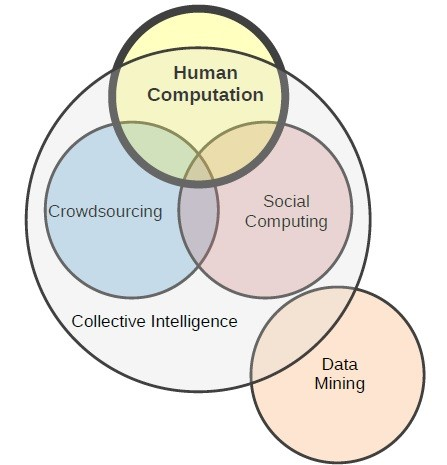
\includegraphics[width=6cm,height=6cm]{graf}

\textbf{Figure 1:}Human computation is a means of solving computational problems. Such problems are found only occasionally in crowdsourcing and social computing applications.
\end{figure}
similarities among various projects. The goal is to reveal the structure of the design space, thus helping new researchers understand the landscape and discover unexplored or underexplored areas of opportunity.

The key contributions can be summarized as follows:
\begin{itemize}
 \item  Human computation is defined concretely and positioned in the context of related techniques and ideas.

\item We give a set of dimensions that can be used to classify and compare existing human computation systems.

\item We explain how to apply the system to identify open opportunities for future research in human computation.
\end{itemize}
\section*{DEFINITION OF HUMAN COMPUTATION}
There have long been many interesting ways that people work with computers, as well as ways they work with each other through computers. This paper focuses on one of them. Human computation is related to, but not synonymous with terms such as \textit{collective intelligence, crowdsourcing}, and \textit{social computing}, though all are important to understanding the landscape in which human computation is situated. Therefore, before introducing our human computation taxonomy itself, we will define a few of these terms, each on its own and in the context of human computation. This is important because without establishing the boundaries of human computation, it would be difficult to design a consistently applicable classification system. Since we have no particular authority over these definitions, we will defer to the primary sources wherever possible.
\section*{Human Computation}
The term \textit{human computation} was used as early as 1838 [69] in philosophy and psychology literature, as well as more recently in the context of computer science theory [62]. However, we are most concerned with its modern usage. Based on historical trends of its use in computer science literature (Figure 2) as well as our examination of citations between papers, it appears that the modern usage was inspired by von Ahn's 2005 dissertation titled "Human Computation" [64] and the work leading to it. That thesis defines the term as:

\textit{"\dots a paradigm for utilizing human processing power to solve problems that computers cannot yet solve."}
\begin{figure}[h]
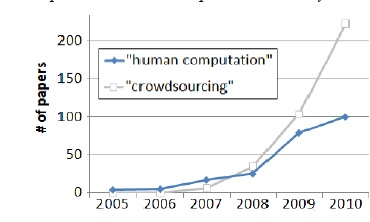
\includegraphics[width=6cm,height=3cm]{graf2}

\textbf{Figure 2:}Use of the terms "human computation" and "crowdsourcing" in the computer science literature has been steadily increasing. Search results for the two terms in the ACM Guide to the Literature were counted on January 14, 2010 and may not include all publications from late 2010.
\end{figure}

This seems compatible with definitions given elsewhere by von Ahn (co-author on the first one) and others (the rest):

\textit{"\dots the idea of using human effort to perform tasks that computers cannot yet perform, usually in an enjoyable manner."} [33]

\textit{"\dots a new research area that studies the process of channeling the vast internet population to perform tasks or provide data towards solving 
difficult problems that no known efficient computer algorithms can yet solve." }~\cite{chandrasekar2010}

\textit{"\dots a technique that makes use of human abilities for computation to solve problems." }[8,74]

\textit{"\dots a technique to let humans solve tasks, which cannot be solved by computers."} [54]

\textit{"A computational process that involves humans in certain steps\dots "} [73]

\textit{"\dots systems of computers and large numbers of humans that work together in order to solve problems that could not be solved by either computers or humans alone"} [50]

\textit{"\dots a new area of research that studies how to build systems, such as simple casual games, to collect annotations from human users."} [34]

Most other papers using the term do not define it explicitly. From these definitions, taken together with the body of work that self-identifies as human computation, a consensus emerges as to what constitutes human computation:
\begin{itemize}
  \item  The problems fit the general paradigm of computation, and as such might someday be solvable by computers.
  \item The human participation is directed by the computational system or process. (This is discussed more below.)
\end{itemize}
\section*{COMPARISON WITH RELATED IDEAS}
The definition and criteria above do not include all technologies by which humans collaborate with the aid of computers, even though there may be intersections with related topics. For example, human computation does not encompass online discussions or creative projects where the initiative and flow of activity are directed primarily by the participants' inspiration, as opposed to a predetermined plan designed to solve a computational problem.

We further argue that editing Wikipedia articles is excluded, though the distinction is subtle. An encyclopedia purist might argue that an online encyclopedia should contain no creative content and could be interpreted as a very advanced search engine or information retrieval system that gathers existing knowledge and formulates it as prose. Such is the goal of Wikipedia's "neutral point of view" policy [71]. If realized fully and perfectly, perhaps Wikipedia might reasonably be considered an example of human computation. However, Wikipedia was designed not to fill the place of a machine, but as a collaborative writing project in place of the professional encyclopedia authors of yore. The current form of Wikipedia is created through a dynamic social process of discussion about the facts and presentation of each topic among a network of the authors and editors [30]. When classifying an artifact, we consider not what it aspires to be, but what it is in its present state.

Perhaps most notably, the very choice of which articles to create is made by the authors, the people who would be counted as part of the computational machinery if Wikipedia editing were considered computation. A computer with free will to choose its tasks would cease to be a computer [62]. Therefore, Wikipedia authors cannot be regarded as merely performing a computation.
\section*{Crowdsourcing}
The term \textit{crowdsourcing},first coined in a Wired magazine article by Jeff Howe [22] and the subject of his book [23], was derived from\textit{outsourcing}. Howe's web site offers the
\begin{wrapfigure}[7]{r}{5cm}
\fbox{\begin{minipage}{\dimexpr\linewidth-2\fboxrule-2\fboxsep}
Whereas         human            computation \\      
replaces        computers        with \\             
humans, crowdsourcing replaces\\
traditional human workers with\\
members of the public.
\end{minipage}}
\end{wrapfigure}
 following definition, which frames it as a replacement for roles that would otherwise be filled by regular workers:
\textit{"Crowdsourcing is the act of taking a job traditionally performed by a designated agent (usually an employee) and outsourcing it to an undefined, generally large group of people in the form of an open call."} [24]

There is some overlap between human computation and crowdsourcing where computers and humans already had established roles performing the same type of task. However, the center of gravity of the two terms is different.

The intersection of crowdsourcing with human computation in Figure 1 represents applications that could reasonably be considered as replacements for either traditional human roles or computer roles. For example, translation is a task that can be done either by machines when speed and cost are the priority, or by professional translators when quality is the priority. Thus, approaches such as our MonoTrans project [2,25], which provides a compromise solution with moderate speed, cost, and quality, could be considered members of both sets.
\section*{Social Computing}
Technologies such as blogs, wikis, and online communities are examples of \textit{social computing}. The scope is broad, but always includes humans in a social role where communication is mediated by technology. The purpose is not usually to perform a computation. Various definitions of social computing are given in the literature:

\textit{"\dots applications and services that facilitate collective action and social interaction online with rich exchange of multimedia information and evolution of aggregate knowledge\dots "} [48]

\textit{"\dots the interplay between persons' social behaviors and their interactions with computing technologies"} ~\cite{cooper2010pre}

The key distinction between human computation and social computing is that social computing facilitates relatively natural human behavior that happens to be mediated by technology, whereas participation in a human computation is directed primarily by the human computation system.
\section*{Data Mining}
Data mining can be defined broadly as:

"\textit{the application of specific algorithms for extracting patterns from data.}" [17]

Since these algorithms are often used to extract patterns from human-created data, some might think of them as a form of human computation. We argue that data mining software in itself does not constitute human computation.

As an example, consider Google's PageRank web indexing algorithm, which mines the structure of hyperlinks between web pages to estimate the relevance of web pages to search queries [47]. Many of the pages were indeed created and linked together by humans. However, the work that the humans did in linking the pages was not caused or directed by the system and, in fact, may have taken place before the PageRank algorithm was even invented. Thus, the system cannot be said to have harnessed their processing abilities. Furthermore, the humans created the pages out of free will, so they cannot be said to be part of a computation.

In general, the use of data mining software does not encompass the collection of the data, whereas the use of human computation necessarily does. Thus, no data mining software system can be human computation, and vice versa.

This distinction matters because if data mining were considered as human computation, our taxonomy would need to be as applicable to data mining applications as it is to the rest of the ideas included in human computation. For example, challenges common to all human computation systems (i.e., resistance to cheating, motivation, etc.) do not make sense when discussed in the context of data mining.
\section*{Collective Intelligence}
Encompassing most of the territory discussed so far is the overarching notion that large groups of loosely organized people can accomplish great things working together. Traditional study of collective intelligence focused on the inherent decision making abilities of large groups [36,42]. However, the view most relevant to human computation is that expressed in Malone’s taxonomical "genome of collective intelligence." It defines the term very broadly as:

\textit{"\dots groups of individuals doing things collectively that seem intelligent."} [41]

Malone's work scope explicitly includes the PageRank algorithm, as well as virtually any group collaboration, even including "families, companies, countries, and armies." Therefore, as Figure 1 illustrates, collective intelligence is a superset of social computing and crowdsourcing, because both are defined in terms of social behavior. Data mining crosses the circle because some applications benefit from groups while others do not (i.e. mining climate data).
The key distinctions between collective intelligence and human computation are the same as with crowdsourcing, but with the additional distinction that collective intelligence applies only when the process depends on a group of participants. It is conceivable that there could be a human computation system with computations performed by a single worker in isolation. This is why part of human computation protrudes outside collective intelligence.

We are unaware of any well-developed examples of human computation that are not collective intelligence, but it is conceivable and might be a basis for some future work. Suppose a solitary human translator operates an on-demand, mechanized translation service. It is human computation because it utilizes the human translator’s abilities to do a computation, translating text from one language to another. It would not be considered collective intelligence because there is no group, and thus no group behavior at work.
\section*{CLASSIFICATION DIMENSIONS}
The common denominator among most human computation systems is that they rely on humans to provide units of work which are aggregated to form an answer to the request. Still, that leaves a wide range of possible structures and algorithms that can (or could) be utilized.

The classification system we are presenting is based on six of the most salient distinguishing factors. These are summarized in Figure 3. For each of these dimensions, we provide a few possible values corresponding to existing systems or notable ideas from the literature. Part of the job of researchers and technologists working to advance human computation will be to explore new possible values to address unmet needs, such as better control over speed and quality, efficient use of workers’ time, and positive working relationships with the humans involved.

To develop the dimensions, we started by performing a review of the human computation literature and notable examples found in industry. Within those examples, we searched for groupings that tend to cite each other, use a common vocabulary, or share some obvious commonality. For example, there is a large cluster in the literature relating to games with a purpose (GWAPs).

For the taxonomy to be valid and useful, every dimension must have at least one (and ideally only one) value for each human computation system. To that end, we identified the underlying properties that these groupings have in common, expressed in a way that would be relevant for any of the examples seen in the initial review. For example, all GWAPs use enjoyment as their primary means of motivating participants. These properties formed three of our dimensions: \textit{motivation, human skill,} and \textit{aggregation}.

To ensure that the dimensions could be used to gain new insight into the field of human computation, we also looked for properties that cut across the more obvious groupings. For example, a certain cross section of human computation systems has in common that all involve dividing up a singlesource request into small slices (i.e. pages of a book, sections of an image, frames of a video, etc.), and issuing each slice as an individual task, even though the rest of the system design and problem domain may be completely different. In this way, three more properties were formed:\textit{quality control, process order,} and \textit{task-request cardinality.}
\section*{Motivation}
One of the challenges in any human computation system is finding a way to motivate people to participate. This is eased somewhat by the fact that most human computation systems rely on networks of unrelated people with connected computers in their homes or workplaces. They need not go anywhere or do anything too far out of their ordinary lives to participate. Even so, since the computations frequently involve small unit tasks that do not directly benefit the contributors, they will only participate if they have a motivation-a reason why doing the tasks is more beneficial to them than not doing them. Unlike a traditional job, which almost always pays with money, human computation workers may be motivated by a number of factors. Still, some workers are paid, so we start there.
\section*{Pay}
Financial rewards are probably the easiest way to recruit workers, but as soon as money is involved, people have more incentive to cheat the system to increase their overall rate of pay. Also, because participants are usually anonymous, they may be more likely to do something dishonest than they would if they were identified.

Mechanical Turk [44] is an online market for small tasks (computational or not) that uses monetary payment. Developers can write programs that automatically submit tasks to be advertised on the site. The tasks are completed by a network of workers, usually directly through the Mechanical Turk web site. Prices are driven by an open market with about 90\% of tasks paying \$0.10 or less [27].

Another example that uses financial motivation is ChaCha ~\cite{chen2010}, a search service that uses humans to interpret search queries and select the most relevant results. LiveOps [40] is a company that employs workers online to handle phone calls for businesses, as a sort of distributed call-center. The workers follow scripts, which makes the job analogous to an automated telephone system, a role that might otherwise be filled by a computer. An older example was the Cyphermint PayCash anonymous payment kiosks [49,18], which used remote human workers to help verify the user's identity.

In some cases, the pay need not be money. CrowdFlower is a company that acts as an intermediary for businesses wanting to take advantage of crowdsourcing or human computation ~\cite{biewald2011}. Businesses send tasks to CrowdFlower, which works with a variety of services for connecting with and compensating workers (i.e., Mechanical Turk, Gambit, Prodege/SwagBucks, TrialPay, etc.). Workers may be paid in money, gift certificates, or even virtual currency redeemable for virtual goods in online games.
\begin{figure*}[t]
\centering
\begin{tabular}{|l|l|l|}
\Xhline{1mm}
\multicolumn{1}{|l|}{\textbf{Dimension}}   & \multicolumn{1}{l|}{\textbf{Sample values}}                    & \multicolumn{1}{l|}{\textbf{Example}}                              \\ \Xhline{1mm}
\multicolumn{1}{|l|}{\textbf{Motivation}}  & \multicolumn{1}{l|}{Pay}                                       & \multicolumn{1}{l|}{Mechanical Turk {[}44{]}}                      \\ \cline{2-3}
\multicolumn{1}{|l|}{\textbf{}}            & \multicolumn{1}{l|}{Altruism}                                  & \multicolumn{1}{l|}{helpfindjim.com (Jim Gray) {[}19{]}}           \\ \cline{2-3}
\multicolumn{1}{|l|}{\textbf{}}            & \multicolumn{1}{l|}{Enjoyment}                                 & \multicolumn{1}{l|}{ESP Game {[}63{]}}                             \\ \cline{2-3}
\multicolumn{1}{|l|}{\textbf{}}            & \multicolumn{1}{l|}{Reputation}                                & \multicolumn{1}{l|}{Volunteer translators at childrenslibrary.org} \\  \cline{2-3}
\textbf{}                                  & Implicit work                                                  & reCAPTCHA {[}68{]}                                                 \\  \Xhline{1mm}
\multicolumn{1}{|l|}{\textbf{Quality}}     & \multicolumn{1}{l|}{Output agreement}                          & \multicolumn{1}{l|}{ESP Game}                                      \\  \cline{2-3}
\multicolumn{1}{|l|}{\textbf{control}}     & \multicolumn{1}{l|}{Input agreement}                           & \multicolumn{1}{l|}{Tag-a-tune {[}33{]}}                           \\  \cline{2-3}
\multicolumn{1}{|l|}{\textbf{}}            & \multicolumn{1}{l|}{Economic models}                           & \multicolumn{1}{l|}{(see {[}18{]})}                                \\  \cline{2-3}
\multicolumn{1}{|l|}{\textbf{}}            & \multicolumn{1}{l|}{Defensive task design}                     & \multicolumn{1}{l|}{(see ~\cite{callison2010})}                                 \\ \cline{2-3}
\multicolumn{1}{|l|}{\textbf{}}            & \multicolumn{1}{l|}{Redundancy}                                & \multicolumn{1}{l|}{reCAPTCHA}                                     \\  \cline{2-3}
\multicolumn{1}{|l|}{\textbf{}}            & \multicolumn{1}{l|}{Statistical filtering}                     & \multicolumn{1}{l|}{(see ~\cite{chen2009})}                             \\  \cline{2-3}
\multicolumn{1}{|l|}{\textbf{}}            & \multicolumn{1}{l|}{Multilevel review}                         & \multicolumn{1}{l|}{Soylent ~\cite{bernstein2015}}                               \\  \cline{2-3}
\multicolumn{1}{|l|}{\textbf{}}            & \multicolumn{1}{l|}{Automatic check}                           & \multicolumn{1}{l|}{fold.it (protein folding game) ~\cite{cooper2010}}       \\  \cline{2-3}
\textbf{}                                  & Reputation system                                              & Mechanical Turk                                                    \\  \Xhline{1mm}
\multicolumn{1}{|l|}{\textbf{Aggregation}} & \multicolumn{1}{l|}{Collection}                                & \multicolumn{1}{l|}{reCAPTCHA}                                     \\  \cline{2-3}
\multicolumn{1}{|l|}{\textbf{}}            & \multicolumn{1}{l|}{Wisdom of crowds}                          & \multicolumn{1}{l|}{Kasparov-World chess game {[}45{]}}            \\  \cline{2-3}
\multicolumn{1}{|l|}{\textbf{}}            & \multicolumn{1}{l|}{Search}                                    & \multicolumn{1}{l|}{helpfindjim.com (Jim Gray)}                    \\  \cline{2-3}
\multicolumn{1}{|l|}{\textbf{}}            & \multicolumn{1}{l|}{Iterative improvement}                     & \multicolumn{1}{l|}{Monotrans ~\cite{hu2010} and {[}39{]}}             \\  \cline{2-3}
\multicolumn{1}{|l|}{\textbf{}}            & \multicolumn{1}{l|}{Genetic algorithm}                         & \multicolumn{1}{l|}{(see {[}32{]})}                                \\  \cline{2-3}
\textbf{}                                  & None                                                           & VizWiz {[}5{]}                                                     \\  \Xhline{1mm}
\multicolumn{1}{|l|}{\textbf{Human skill}} & \multicolumn{1}{l|}{Visual recognition}                        & \multicolumn{1}{l|}{ESP Game}                                      \\  \cline{2-3}
\multicolumn{1}{|l|}{\textbf{}}            & \multicolumn{1}{l|}{Language understanding}                    & \multicolumn{1}{l|}{Soylent}                                       \\  \cline{2-3}
\textbf{}                                 & Basic human communication                                      & ChaCha {[}7{]}                                                     \\  \Xhline{2\arrayrulewidth}
\multicolumn{1}{|l|}{\textbf{Process}}     & \multicolumn{1}{l|}{Computer \carrow Worker \carrow Requester} & \multicolumn{1}{l|}{reCAPTCHA}              \\  \cline{2-3}
\multicolumn{1}{|l|}{\textbf{order}}       & \multicolumn{1}{l|}{Worker \carrow Requester \carrow Computer}             & \multicolumn{1}{l|}{ESP Game}                                      \\  \cline{2-3}
\multicolumn{1}{|l|}{\textbf{}}            & \multicolumn{1}{l|}{Computer \carrow Worker \carrow Requester \carrow Computer}  & \multicolumn{1}{l|}{FACTory {[}60{]}}                              \\  \cline{2-3}
\textbf{}                                  & Requester \carrow Worker                                             & VizWiz                                                             \\  \Xhline{1mm}
\multicolumn{1}{|l|}{\textbf{Task-}}       & \multicolumn{1}{l|}{One-to-one}                                & \multicolumn{1}{l|}{ChaCha}                                        \\  \cline{2-3}
\multicolumn{1}{|l|}{\textbf{Request}}     & \multicolumn{1}{l|}{Many-to-many}                              & \multicolumn{1}{l|}{ESP Game}                                      \\  \cline{2-3}
\multicolumn{1}{|l|}{\textbf{Cardinality}} & \multicolumn{1}{l|}{Many-to-one}                               & \multicolumn{1}{l|}{helpfindjim.com (Jim Gray)}                    \\  \cline{2-3}
\multicolumn{1}{|l|}{\textbf{}}            & \multicolumn{1}{l|}{Few-to-one}                                & \multicolumn{1}{l|}{VizWiz}                                        \\ \Xhline{1mm}
\end{tabular}

\textbf{Figure 3:}Overview of our classification system for human computation systems.
\end{figure*}

\section*{Altruism}
Do good. It may sound easy to trust in people's desire to help, but it can only work if participants actually think the problem being solved is interesting and important.

When the computer scientist Jim Gray went missing during a sailing trip in early 2007, thousands of online volunteers combed through over 560,000 satellite images [19] hoping to determine Gray's location. Sadly the effort was not successful, but the heroic efforts of these volunteers nevertheless demonstrated that people will expend significant time and effort for the right cause.
\section*{Enjoyment}
The abundance of time-consuming, entertainment activities on the Internet attests that even simple forms of entertainment have value to many web users. By making a task entertaining, either as a game or some other enjoyable activity, it is possible to engage humans to do tasks that contribute to a computational goal.

Games With A Purpose is a strategy where you create a game that requires players to perform some computation in order to get points or succeed. People play because they enjoy it. If the game is fun, they may play for a very long time and supply a lot of computational power. However, it can be difficult to turn computational tasks into games that are truly fun to play [65]. Furthermore, it is important to be able to prove that the game will yield correct results, much like designing a computer algorithm [66]. Some views of human computation are centered on the use of games [74]. Games have been created for a variety of computations, including image labeling [63], protein folding ~\cite{cooper2010pre}, and music recognition [33].
\section*{Reputation}
Where the problem is associated with an organization of some prestige, human workers may be motivated by the chance to receive public recognition for their efforts. This strategy has been implemented by the International Children's Digital Library to recruit volunteer translators.
\section*{Implicit work}
It is sometimes possible to make the computation a natural part of some activity the users were already doing. However, examples are scarce because it is very difficult to match a task to an existing activity.
ReCAPTCHA [52,68] is a human computation system for transcribing old books and newspapers for which OCR is not very effective. It takes advantage of the pre-existing need for CAPTCHAs, the distorted images of text that are used by websites to prevent access by automated programs. When a user goes to a website (i.e. a webmail service), instead of seeing computer generated distorted text, they see an image of a word from an old book or newspaper, for which the OCR software could not identify the content. By typing the letters in the course of visiting the website, the user provides computational power to help with the transcription effort.
\section*{Quality control}
Even if the users are motivated to participate, they may try to cheat or sabotage the system. Workers may also be acting in good faith, but misunderstand the directions or make mistakes due to personal bias or lack of experience with the subject matter. Ipeirotis used expectation maximization to estimate the quality, and also infer some characteristics of the types of errors [29].
Output agreement [66]
Epitomized by the ESP game [63] (a game for labeling images), two or more contributors work independently and simultaneously in different locations. The answer is only accepted if the pair can agree on the same answer.
\section*{Input agreement [66]}
This is almost the converse of output agreement. Two humans working independently and simultaneously in different locations are given inputs that may or may not be the same. They are asked to describe the inputs to one another and then try to decide whether they are looking at the same input or different inputs. If both participants agree, then the description is deemed to be correct.

Input agreement was introduced by Law with the Tag-a-Tune game [33], which collects descriptions of music clips. The players each listen to a sound file and type descriptions. If both players agree on whether or not the other’s descriptions seem to be describing the same clip, then the descriptions are deemed to be relevant.
\section*{Economic models}
When money is used as a motivating factor, it may be possible to use different incentive structures to elicit more good quality work for less money [43]. Gentry et al proposed to pay according to a game-theoretic model of the worker's rating, reducing the incentive to cheat [18].
\section*{Defensive task design}
More practically, several solutions have been developed to improve the accuracy of results from paid services like Mechanical Turk [44]. One approach is to design tasks so it is no easier to cheat than to do the task ~\cite{callison2010}.
\section*{Reputation system}
In some systems, users may be motivated to provide quality answers by a reputation scoring system. With Mechanical Turk, a worker who frequently submits bad work can be blocked from accessing future tasks or, more positively, given special access to more desirable tasks.
\section*{Redundancy}
By finding more contributors, you can have each task done by multiple workers, and use a voting scheme to identify good answers. This in turn helps you identify consistently poor workers so that their work can be removed so it does not affect the final quality. In our experience using Mechanical Turk, a large proportion of bad work comes from a small number of human workers.
\section*{Ground truth seeding}
A common approach used by users of Mechanical Turk is to start with a small number of tasks for which ground truth has been provided by a trusted source. By mixing in questions with known answers, the system can identify workers who are deliberately submitting useless answers, or perhaps just confused by the instructions.
\section*{Statistical filtering}
Filter or aggregate the data in some way that removes the effects of irrelevant work. For example, Chen discounts results that do not fit an expected distribution ~\cite{chen2009}.
\section*{Multilevel review}
One set of workers does the work, and a second set reviews the work and rates its quality. It is like output agreement, except that the work need not be done synchronously. More elaborate multilevel schemes are possible, such as the \textit{find-fix-verify} pattern demonstrated by Soylent, a word processor that uses workers on Mechanical Turk to help writers improve their text ~\cite{bernstein2015}.
\section*{Expert review}
A trusted expert skims or cross-checks contributions for relevance and apparent accuracy. For example, with Mechanical Turk, people who post tasks may review the work and choose whether to pay or not.
\section*{Automatic check}
Some problems are much easier to verify than compute. This class of problems lends itself to automatic checking. For example, in automated planning, a subfield of AI, it is difficult for a computer to generate a plan that gets from the start state to a desired end state, but given a plan as input, it is easy to test if it is correct. In the foldit game, users use a graphical interface to predict protein structures, an important problem in biochemistry. The game uses \textit{Rosetta energy} a property of protein structures, to identify the most useful results ~\cite{cooper2010}.
\section*{Aggregation}
Part of the process of human computation is to combine all of the contributions to solve the global problem. The means of doing this partly determines the class of problems a system or strategy can be applied to.
\section*{Collection}
A knowledge base of discrete facts or a hierarchical ontology is collected. A contribution may either add a new fact or improve quality by correcting, refuting, or confirming existing facts in the knowledge base.

Knowledge Collection from Volunteer Contributors (KCVC) is kind of human computation that uses the collection method of aggregation. KCVC is summarized in ~\cite{chklovski2005t}. The goal is to advance artificial intelligence research by using humans to build large databases of common sense facts. The idea is that humans, by way of their child development and adult lives, acquire a great deal of common sense knowledge (i.e. "People cannot brush their hair with a table."). Several efforts have demonstrated ways of using volunteer contributors to provide such facts, either by using games (e.g. the FACTory [60], Verbosity [67], 1001 Paraphrases ~\cite{chklovski2005} ) or by plain volunteerism (e.g. Learner ~\cite{chklovski2003}, Open Mind Common Sense [58]). The collected facts are often used to improve on the results of automated attempts at extracting the information. As such, the practice of KCVC is important to AI research and has been the topic of dedicated workshops and symposia.
\section*{Statistical processing of data}
Consider a game where hundreds of people try to guess the number of jelly beans in a large jar. It turns out that under normal circumstances, the average of the guesses will be very close to the actual count.

In the book, The Wisdom of Crowds, Surowiecki explains how aggregating answers from a decentralized, disorganized group of people, all thinking independently can yield surprisingly accurate results to questions that would be difficult for one person to answer alone. It works only if the individual errors of each person are uniformly distributed, which in turn requires individual judgments to be made independently [59].

Several online polling web sites and prediction markets harness this concept to not only determine a group opinion, but to try to predict future events [72] (e.g. Ask500People~\cite{mcardletermtalk}, News Futures [46], and Iowa Electronic Markets [26]). While prediction markets are not examples of human computation, they are one of the most commonly cited examples of Wisdom of Crowds.
\section*{Iterative improvement}
For some applications, it makes sense to give each worker the answer given by previous workers for the same task. As a test of this strategy, Little asked workers on Mechanical Turk to try to read some text that had been severely distorted for purposes of the experiment [39]. Initially, the image of distorted text was given to two workers. Next, a third worker (or small group of workers) examined the transcriptions from the first two workers, and chose the best one, which was given to the fourth worker as a starting point. They found that iterative improvement had the potential to yield very high quality results, but that the quality was less consistent than the control method they compared with.
\section*{Active learning}
In machine learning, classifiers are software modules that can be trained to recognize certain patterns in data (i.e., outlines of common objects in an image, fraudulent credit card transactions, spoken words, etc.). The simplest way to train a classifier is to input a large quantity of example patterns along with annotations (answers) for it to learn from. Sometimes when obtaining enough annotations would be especially labor-intensive, the active learning approach can be employed to reduce the number of annotations needed to train. The classifier is given a large number of example patterns without annotations. Then, it analyzes them to identify which examples would have the most training benefit if annotations were made available [61]. Human participants then create the annotations, which are given as input to the classifier.

Essentially, the annotations contributed by the human participants are aggregated by the classifier to compute the internal classifier state that will eventually be able to recognize the patterns automatically.
\section*{Search}
Several projects have used large numbers of volunteers to sift through photographs or videos, searching for some desired scientific phenomenon, person, or object.

For example, the Space Sciences Laboratory at the University of California at Berkeley used human computation to search for tiny matter from space as part of the Stardust@home project [70]. The particles had been mixed into an aerogel collector from the Stardust spacecraft. Contributors searched through photographs of the aerogel for traces of the particles. This recognition problem was much too difficult for computer vision algorithms or even untrained humans. Therefore, participants had to complete an online training program to learn how to identify the tiny particles before they could contribute. With this aggregation method, the only contributions that are of value are the one(s) that contain the target (e.g., photo of Jim Gray or trace of a particle).
\section*{Genetic algorithm}
Genetic algorithms are used in computer science to solve search and optimization problems. The Free Knowledge Exchange is a site where users work together to evolve answers to freeform questions. While not actually a computation, it demonstrates how users can perform the key functions of initialization, mutation, and recombinant crossover [32]. A simpler example is PicBreeder, where users evolve interesting graphical patterns by choosing among computer-generated choices [55]. This is probably not computation either, since the choices are subjective.
\section*{None}
Some human computation systems need no aggregation at all, but simply use humans to perform a large number of small tasks which are independent of one another.
\section*{Human Skill} 
Depending on the application, human computation may leverage a variety of skills that are innate to nearly all humans or, in some cases, special knowledge or abilities held by only some (e.g., can read and write Chinese). When designing a solution that uses human computation, it is helpful to be very specific about what skill is being used, in order to factor out other aspects of the problem that could just as easily be done by a computer. For example, to improve an image search engine, one could imagine employing an extremely large number of humans to search through images exhaustively for every query. It is far more efficient to have them simply associate text descriptions with images, and then have a computer search the text.
\section*{Process Order}
In any human computation system, there are three roles: the requester, worker, and computer. The requester is the end user who benefits from the computation (i.e., someone using an image search engine to find something). A subtle distinction among human computation systems is the order in which these three roles are performed. We consider the computer to be active only when it is playing an active role in solving the problem, as opposed to simply aggregating results or acting as an information channel. Many permutations are possible.
\section*{Computer \carrow Worker \carrow Requester (CWR)}
With reCAPTCHA [68], a \textit{computer} first makes an attempt to recognize the text in a scanned book or newspaper using OCR. Then, words which could not be confidently recognized are presented to web users (\textit{workers}) for help. Their transcriptions become part of the transcription of the book or newspaper for use by users (\textit{requesters}) reading or listening to it.
\section*{Worker \carrow Requester \carrow Computer (WRC)}
Players (\textit{workers}) of image labeling games [63, etc.] provide labels for images, which are then aggregated by a computer to remove labels believed to be irrelevant. When a web user (\textit{requester}) visits the image search site and enters a query, the \textit{computer} searches the database of labels to find matches.

\section*{Computer \carrow Worker \carrow Requester \carrow Computer (CWRC)}
The Cyc system (\textit{computer}) has inferred a large number of common sense facts by analyzing text. To improve the quality of the facts in the database, they use FACTory [60], a game with a purpose. Facts from the database are presented to players (\textit{workers}) who can confirm or correct them, thus improving the quality of the Cyc database. When an user (\textit{requester}) of Cyc performs a query that requires AI functionality, the system (\textit{computer}) make inferences using facts in the database.
\section*{Requester \carrow Worker (RW)}
Mechanical Turk [44] allows a \textit{requester} to submit tasks, such as audio transcription or text dictation, for which no additional computation is necessary. For small jobs, quality can be confirmed by spot checking.
\section*{Task-request cardinality}
When an end-user uses a service powered by human computation, there may be many human workers involved in producing the result, especially if a lot of aggregation is required. In other cases, just one or a handful of workers may suffice. This depends on the structure of the problem, and thus is a key dimension in classifying human computation systems, as well as analyzing the financial or time requirements of any given system.
\section*{One-to-one}
With ChaCha’s web search a single human worker would handle the entire search. (Recently, ChaCha changed to a multi-stage process for their SMS mobile search service.)
\section*{Many-to-many}
Image search engines use tagging done by many humans to annotate each image in the search index, which is then used to process any number of search requests. Without receiving several annotations for each of a very large number of images, it would be impossible to return results for any single query.
\section*{Many-to-one}
In the search for Jim Gray, over 12,000 [57] volunteers attempted to find just one image out of over 560,000.
\section*{Few-to-one}
VizWiz ~\cite{bigham2010} is a mobile application that lets a blind user take a photo (i.e., restroom doors) and ask a question (i.e., Which is the men's room?). A few workers on Mechanical Turk give redundant answers to each query.
\section*{OPENINGS FOR GROWTH}
Up to this point, we have described a classification system that can be used to understand human computation systems in the broader context of what exists. We are now ready to use the dimensions to presuppose some possible areas for future exploration. The examples mentioned so far occupy specific points in the design space, but by combining the dimensions in other ways, it is possible to imagine new kinds of systems that could be used to solve other problems.
\section*{Consider new dimension pairs}
For researchers looking for new avenues within human computation, a starting point would be to pick two dimensions and list all possible combinations of values. For example, considering motivation and aggregation shows that input agreement has not been applied with paid labor or any motivation other than enjoyment. Similarly, combining cardinality with motivation reveals that there are no known examples of one-to-one human computation motivated by altruism. One might imagine a service like VizWiz that used trusted volunteers so that redundancy was not needed.

\section*{Invent new values for dimensions}
Another way to use a classification system is to consider if there are other possible values that could be used for a given dimension. For example, one might look for human skills that have not yet been well-explored. The foldit protein folding game made use of humans' spatial manipulation abilities, a skill that still has not been well utilized in other human computation systems~\cite{cooper2010pre}.
\section*{Classify new work and consider variations}
When encountering new work, it may be helpful to think of the applicable values for each dimension of the system. Doing this may help identify ways in which the novel aspect of the system could be combined with other ideas. For example, when encountering the VizWiz mobile application, one might note that it uses pay for motivation, few-to-one cardinality, and a Requester$\rightarrow$Worker (RW) process order. Changing the process order to (CRW) might yield an interesting application that uses the mobile device's CPU to do more meaningful processing before the request is ever entered into the phone. Perhaps it could use situational awareness to suggest possible requests.
\section*{CONCLUSIONS}
Our motivation in developing this classification system was to stimulate new directions of research in human computation. Many researchers and practitioners are excited about this new area within HCI, but there can be a tendency to focus on just one style of human computation, potentially missing more suitable solutions to a problem.

Beyond new algorithms and designs, there is also a pressing need to address issues related to ethics and labor standards. It is possible that as technology obviates the jobs of some unskilled workers, future human computation systems may offer a viable employment option for them. The current state of human computation has a tendency to represent workers as faceless computational resources. As designers, we have the power to orient our systems to encourage positive working arrangements and fair pay as the default.

Finally, the first two sections addressed distinctions between terms in some detail. While it is important as a community to agree on a vocabulary, it is equally important to consider what is left out. Perhaps future incarnations will be more social in nature, while still maintaining their purpose as systems for performing computations.
\section*{ACKNOWLEDGMENTS}
We gratefully acknowledge the advice and support of Lise Getoor, Chang Hu, Pete Kelleher, Oded Nov, Ben Shneiderman, Alexander Sorokin, and Yan Xu.

\bibliographystyle{abbrv}
\bibliography{referencie}

\balancecolumns
\end{document}
